%%%%%%%%%%%%%%%%%%%%%%%%%%%%%%%%%%%%%%%%%%%%%%%%%%%%%%%%%%%%%%%%
%%%%%%%%%%%%%%%%%%%%%%%%%%%%%%%%%%%%%%%%%%%%%%%%%%%%%%%%%%%%%%%%
%%%%%%%%%%%%%%%%%%%%%%%%%%%%%%%%%%%%%%%%%%%%%%%%%%%%%%%%%%%%%%%%

\newpage

\eglabel{6}
\section{Example \theexamples: Joint PKPD model with count data}
\label{sec:eg6}
The following example features a new aspect of the \pml, the support of discrete 
data model, here one using the Poisson distribution to describe count data\footnote{The 
example is encoded in \xatt{example6\_NONMEM.xml} with design sourced 
from a NONMEM datafile.}, based on the MLXTRAN tutorial, 
\cite{Monolix4.3Tutorial:2014}.
%%%%%%%%%%%%%%%%%%%%%%%%%%%%%%%%%%%%%%%%%%%%%%%%%%%%%%%%%%%%%%%%
\subsection{Description}
\label{subsec:exp6_intro} 
The essential bit of information for this task is the probability distribution of count 
data Y, which can be defined in either un-transformed, P(Y=k), or transformed, 
log(P(Y=k)), form. 
We assume the basic Poisson model defined in eq. (\ref{eq:poissonModel}). 
As in example \ref{sec:eg1}, the underlying PK model is 1-compartmental oral model. 
Then we estimate the log-likelihood that the outcome is k using the non-homogeneous 
Poisson model 
\begin{eqnarray}
&& P\big(Y_{\iijj}=k | \Cc_{\iijj}, \psi_i\big) =  \frac{e^{-\lambda_{\iijj}} \lambda^k_{\iijj}}{k!} \label{eq:poissonModel}
\end{eqnarray}
with concentration dependent mean $\lambda$, defined in eq.\ref{eq:lambdasurface},
\begin{eqnarray}
&& \lambda_{\iijj} = \lambda_0 \Big(1 - \frac{\Cc_{\iijj}}{IC_{50} + \Cc_{\iijj}}\Big)  \label{eq:lambdasurface}
\end{eqnarray}
also called Poisson intensity. Here, $\lambda$, depends on the parameters 
$\lambda_0$ and $IC_{50}$ which are sampled from log-normal distribution. 
$\lambda_0$, stands here for the baseline seizure count prior to any drug. 
The value of $\lambda$ is reduced by the concentration in the central 
compartment, $\Cc$, which is visualised for three different values 
of $\Cc = \{1,5,15\}$ in \ref{fig:lambdasurface} ($1\equiv$ green, $5 \equiv$ 
red, $15 \equiv$ blue).

\begin{figure}[htbp]
\centering
\begin{tabular}{cc}
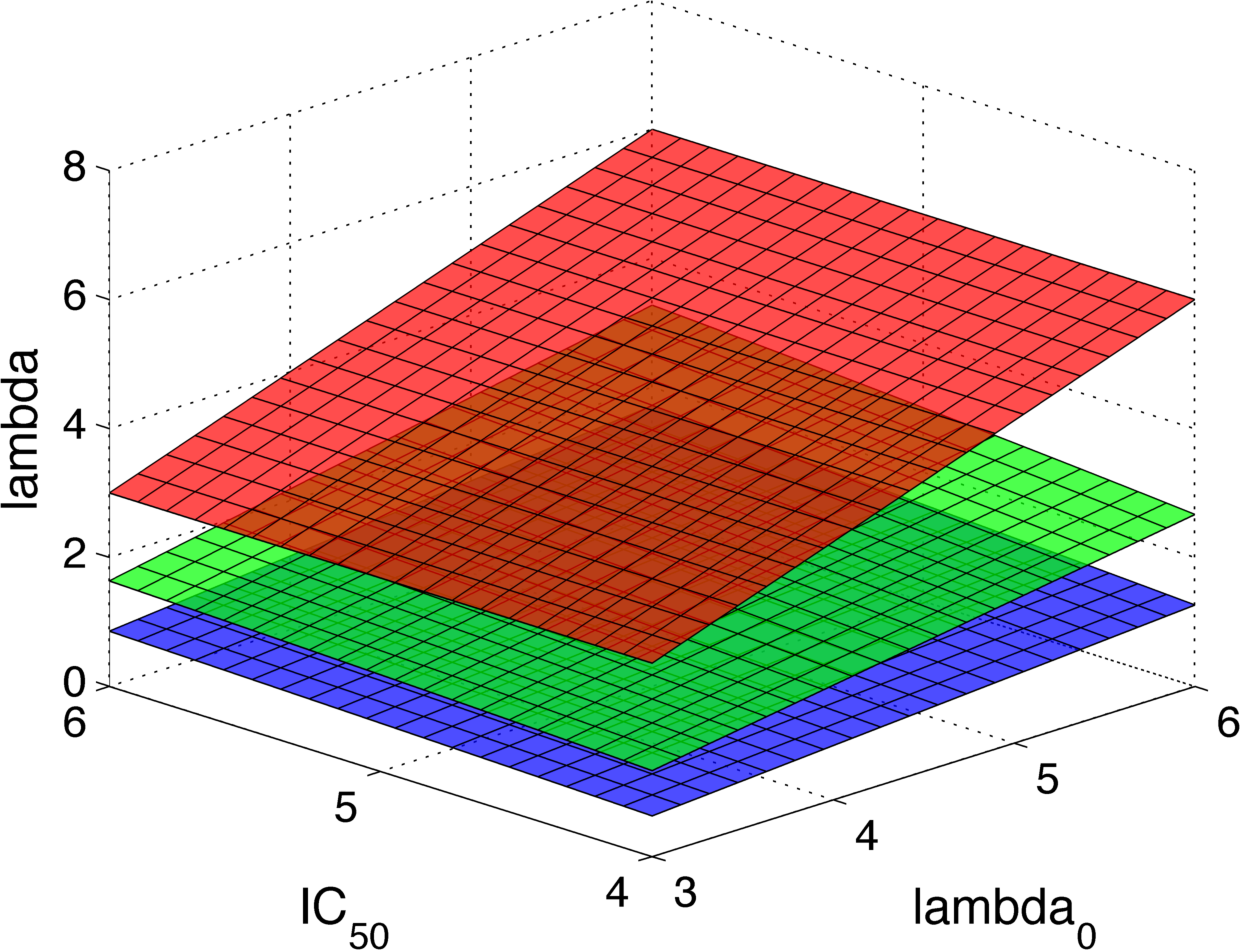
\includegraphics[width=.43\textwidth]{pics/CTS4_lambda_threeSurfaces} & 
\raisebox{0\height}{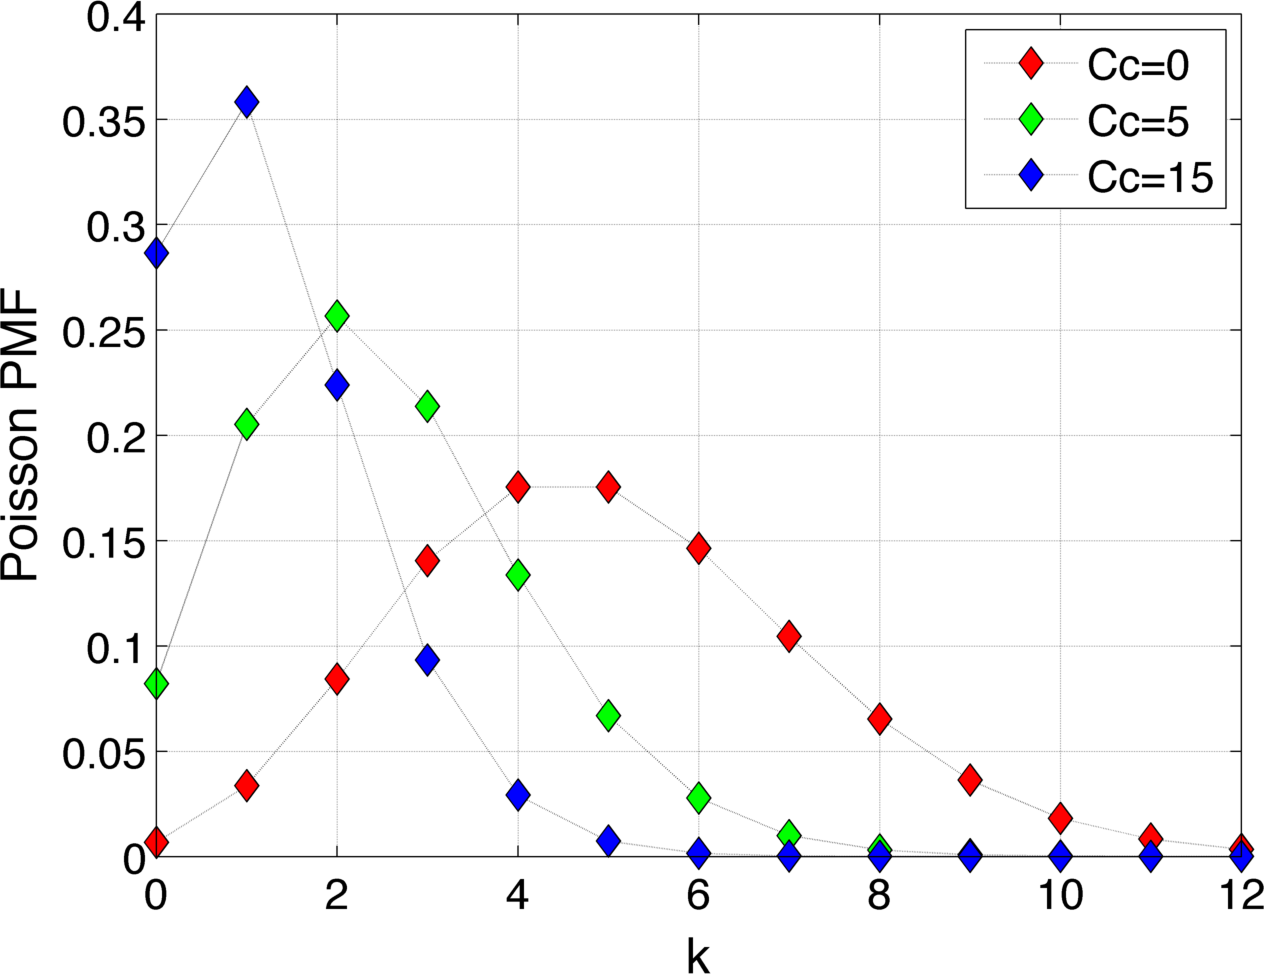
\includegraphics[scale=0.45]{pics/CTS4_poissonScan}}
\end{tabular}
\caption{(left) $\lambda$--surface as function of $\lambda_0$ and $IC_{50}$ 
plotted for $\Cc = \{1,5,15\}$. (right) Poisson PMF for fixed parameters 
$\lambda_0 = IC_{50} = 5$ and varying concentration $\Cc = \{1,5,15\}$.}
\label{fig:lambdasurface}
\end{figure}

\subsubsection{Individual parameters model}
\begin{eqnarray}
\lambda_0 & \sim&  \mbox{logNormal}(\pop_{\lambda_0}, \omega_{\lambda_0}); \quad  \pop_{\lambda_0} = 5, \quad \omega_{\lambda_0} = 0.2 \nonumber \\
IC_{50} &\sim& \mbox{logNormal}(\pop_{IC_{50}}, \omega_{IC_{50}}); \quad  \pop_{IC_{50}} = 5, \quad \omega_{IC_{50}} = 0 \nonumber
\end{eqnarray}

\begin{figure}[htbp]
\centering
\begin{tabular}{cc}
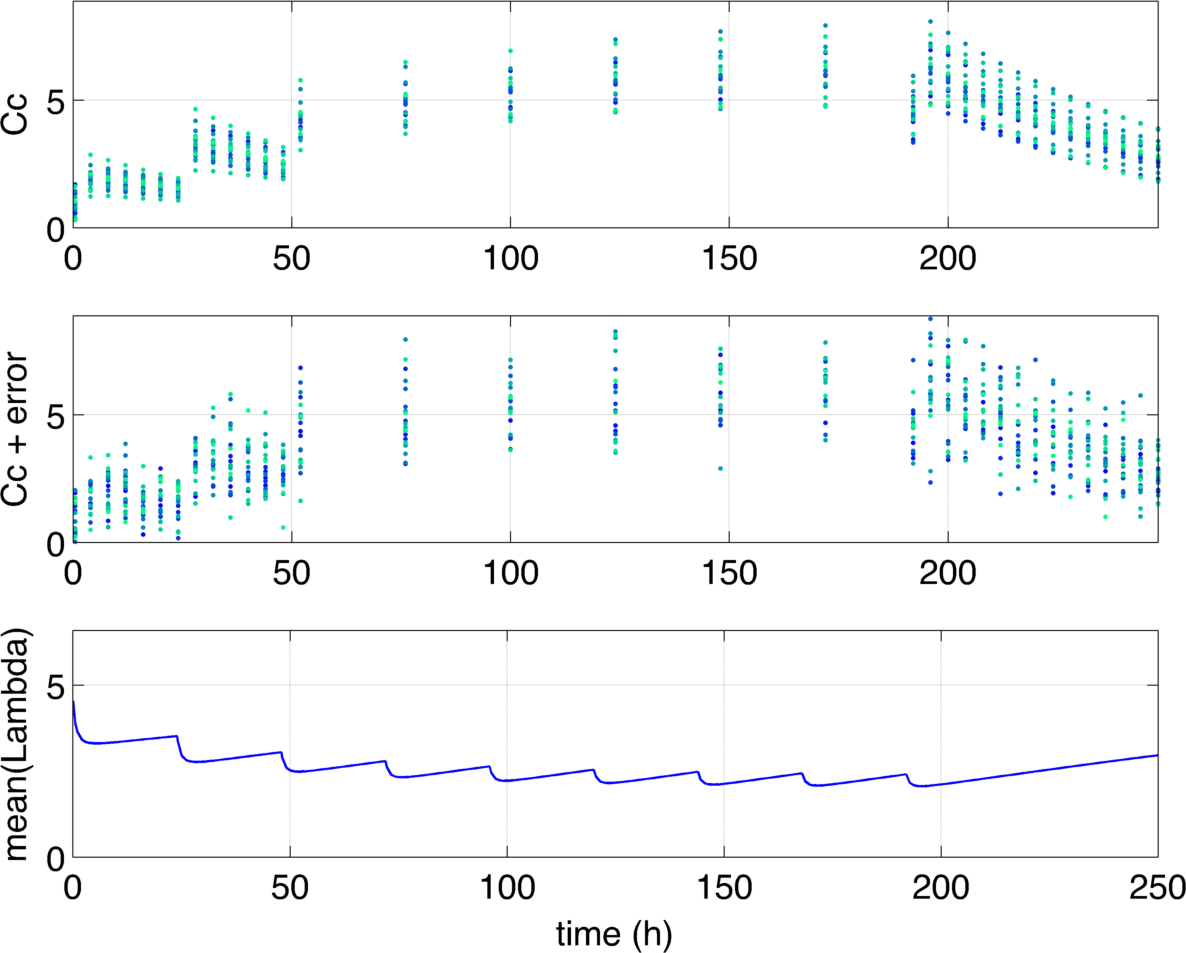
\includegraphics[width=.49\textwidth]{pics/CTS4_PK_meanLambda_armB} & 
\raisebox{0.05\height}{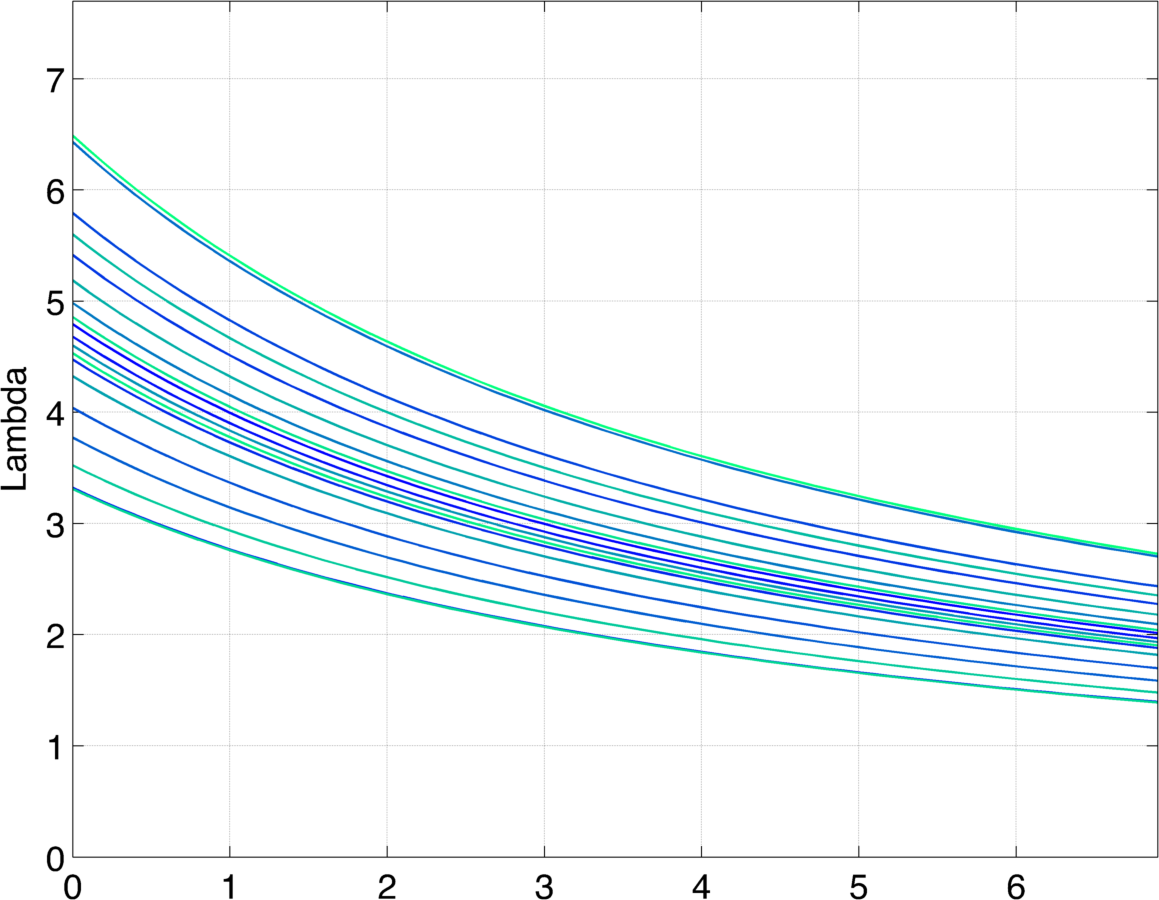
\includegraphics[scale=0.4875]{pics/CTS4_lambda}}
\end{tabular}
\caption{(left) . (right) .}
\label{fig:lambdasurface}
\end{figure}
\marginpar{CORRECT CAPTION IN FIGURE}
\marginpar{\HandCuffLeft}
\marginpar{CORRECT CAPTION}


\subsubsection{Observation model}
We apply a residual error model to the output variables \var{Cc} and \var{E}
from the PK and PD models respectively.

%\begin{table*}[h!]
\begin{center}
\begin{tabular*}{0.8\linewidth}{@{\extracolsep{\fill}} >{\bfseries}l l l}\toprule
Output Variable & \textbf{\itshape Cc} &\textbf{\itshape Y}\\\midrule
Observation Name & Concentration & State \\
Units & $\mg/l$ & -- \\
Type & Continuous & Discrete/Count \\
Model & Combined & Poisson\\
Parameters 	& $a, b$ 	& $\lambda_0, IC_{50}$\\
%Regressor	& --		& $Cc$ \\
\bottomrule
\end{tabular*}
\end{center}
Two additional important bits of information to be provided are 
\begin{itemize}
\item
Intensity Parameter, $\lambda$, given by eq. (\ref{eq:lambdasurface})
\item
Link function -- $\log$
\end{itemize}


\subsection{Observation model}
While the continuous observation model and its features as applied for example 
for the concentration has been described in very detail in the previous examples,
the error distribution of the discrete effect given by eqs.(\ref{eq:poissonModel}) 
and (\ref{eq:lambdasurface}) will be described in the following for the first time.

First we have to indicate the type of the observation model using the elements 
\xelem{Discrete} and specifically for this example \xelem{CountData}. The next 
mandatory element is \xelem{CountVariable} required for the mapping between 
the model and the related date set, see Table \ref{tab:example6_dataSet}. 
Then the characteristic parameter for the Poisson distribution is implemented, the 
\emph{Poisson intensity}, $\lambda$, as function of the drug concentration, $Cc$.

\lstset{language=XML}
\begin{lstlisting}
        <ObservationModel blkId="om1">
            <Discrete>
                <CountData>
                    <ct:Variable symbolType="int" symbId="k"/>
                    <CountVariable symbId="Y"/>
                    
                    <!-- Poisson intensity - function of drug concentration, Cc -->                    
                    <IntensityParameter symbId="Lambda">
                        <ct:Assign>
                            <math:Equation>
                                <math:Binop op="times">
                                    <ct:SymbRef blkIdRef="pm1" symbIdRef="lambda0"/>
                                    <math:Binop op="minus">
                                        <ct:Real>1</ct:Real>
                                        <math:Binop op="divide">
                                            <ct:SymbRef blkIdRef="sm1" symbIdRef="Cc"/>
                                            <math:Binop op="plus">
                                                <ct:SymbRef blkIdRef="pm1" symbIdRef="IC50"/>
                                                <ct:SymbRef blkIdRef="sm1" symbIdRef="Cc"/>
                                            </math:Binop>
                                        </math:Binop>
                                    </math:Binop>
                                </math:Binop>
                            </math:Equation>
                        </ct:Assign>
                    </IntensityParameter>
                    <!-- see next listing for the continuation of the observation model -->
\end{lstlisting}
Now the Poisson probability mass function (PMF) needs to be defined, which can be done
in various ways, either
\begin{itemize}
\item
using the UncertML standard as in the following snippet
\lstset{language=XML}
\begin{lstlisting}
                    <!-- P(Y=k) = exp(-lambda) * lambda^k / k! using UncertML -->
                    <PMF linkFunction="log">
                        <PoissonDistribution xmlns="http://www.uncertml.org/3.0" 
                            definition="http://www.uncertml.org/3.0">
                            <rate>
                                <var varId="Lambda"/>
                            </rate>
                        </PoissonDistribution>
                    </PMF>
                </CountData>
            </Discrete>
        </ObservationModel>
\end{lstlisting}
\item
by encoding explicitly the PMF in the transformed format 
\begin{align}
\log(P\big(Y_{\iijj} & =k | \Cc_{\iijj}, \psi_i\big)) =  -\lambda_{\iijj} +k\times \lambda_{\iijj} - \log(k!) \nonumber
\end{align}

and specifying the
the applied link function, here the logarithm, as the following snippet shows
\lstset{language=XML}
\begin{lstlisting}
                    <!-- log(P(Y=k)) = -Lambda + k*log(Lambda) - log(k!) -->
                    <PMF linkFunction="log">
                        <math:LogicBinop op="eq">
                            <ct:SymbRef symbIdRef="Y"/>
                            <ct:SymbRef symbIdRef="k"/>
                        </math:LogicBinop>
                        <ct:Assign>
                            <Equation xmlns="http://www.pharmml.org/pharmml/0.6/Maths">
                                <Binop op="minus">
                                    <Binop op="plus">
                                        <Uniop op="minus">
                                            <ct:SymbRef symbIdRef="Lambda"/>
                                        </Uniop>
                                        <Binop op="times">
                                            <ct:SymbRef symbIdRef="k"/>
                                            <Uniop op="log">
                                                <ct:SymbRef symbIdRef="Lambda"/>
                                            </Uniop>
                                        </Binop>
                                    </Binop>
                                    <Uniop op="factln">
                                        <ct:SymbRef symbIdRef="k"/>
                                    </Uniop>
                                </Binop>
                            </Equation>
                        </ct:Assign>
                    </PMF>
                </CountData>
            </Discrete>
        </ObservationModel> 
\end{lstlisting}
\end{itemize}

Note, that although the UncertML driven solution is very simple and straightforward
to implement, it is also limited due the reasons explained in Section 
\ref{subsec:DiscreteData}. In short, for count data models, only Poisson model is 
available for now in the  UncertML standard.


%%%%%%%%%%%%%%%%%%%%%%%%%%%%%%%%%%%%%%%%%%%%%%%%%%%%%%%%%%%%%%%%
\subsection{NONMEM dataset}
\label{sec:eg6-NONMEMdataset}
The remaining part is the the data and trial design as sourced from the 
NONMEM dataset. Table \ref{tab:example6_dataSet} show a typical dataset required for 
an estimation task.
\begin{table}[htdp]
\begin{center}
\small
\begin{tabular}{rrrrrrrr}\toprule
ID 	& TIME	& AMT	& Y		& DVID \\ \midrule
1 	& 0 		& 100 	& . 		& . \\ 
1 	& 4 		& . 		& 9.2 	& 1 \\ 
1 	& 8 		& . 		& 5 		& 2 \\ 
1 	& 12 	& . 		& 8.5 	& 1 \\ 
1 	& 18 	& . 		& 6.4 	& 1 \\ 
1 	& 24 	& . 		& 2 		& 2 \\ 
2 	& 0 		& 120	&  26 	& . \\ 
2 	& 4 		& . 		& 4.8 	& 1 \\ 
2 	& 8 		& . 		& 3 		& 2 \\ 
2 	& 12 	& . 		& 3.1 	& 1 \\ 
2 	& 18 	& . 		& 2.5 	& 1 \\ 
2 	& 24 	& . 		& 0 		& 2 \\ 
...	& ...		& ...		& ...		& ...	\\ \bottomrule
\end{tabular}
\end{center}
\caption{A dataset used in example for first two subjects.
The additional column DVID is used to specify the type of data. Here, 
DVID =1 is used for a continuous response and DVID =2 for count data.}
\label{tab:example6_dataSet}
\end{table}%

\marginpar{CORRECT MAPPING DESCRIPTION}



\lstset{language=XML}
\begin{lstlisting}
        <mstep:ExternalDataSet toolName="NONMEM" oid="NMoid">
            <mstep:ColumnMapping>
                <ds:ColumnRef columnIdRef="TIME"/>
                <ct:SymbRef symbIdRef="t"/>
            </mstep:ColumnMapping>
            <mstep:ColumnMapping>
                <ds:ColumnRef columnIdRef="AMT"/>
                <ct:SymbRef blkIdRef="sm1" symbIdRef="Ad"/>
            </mstep:ColumnMapping>
            <mstep:MultipleDVMapping>
                <ds:ColumnRef columnIdRef="DV"/>
                <mstep:Piecewise>
                    <math:Piece>
                        <ct:SymbRef blkIdRef="om1" symbIdRef="Y"/>
                        <math:Condition>
                            <math:LogicBinop op="eq">
                                <ds:ColumnRef columnIdRef="EVID"/>
                                <ct:Real>1</ct:Real>
                            </math:LogicBinop>
                        </math:Condition>
                    </math:Piece>
                    <math:Piece>
                        <ct:SymbRef blkIdRef="om2" symbIdRef="C_obs"/>
                        <math:Condition>
                            <math:LogicBinop op="eq">
                                <ds:ColumnRef columnIdRef="EVID"/>
                                <ct:Real>2</ct:Real>
                            </math:LogicBinop>
                        </math:Condition>
                    </math:Piece>
                </mstep:Piecewise>
            </mstep:MultipleDVMapping>
            <ds:DataSet>
                <ds:Definition>
                    <ds:Column columnId="ID" columnType="id" valueType="string" columnNum="1"/>
                    <ds:Column columnId="TIME" columnType="idv" valueType="real" columnNum="2"/>
                    <ds:Column columnId="AMT" columnType="dose" valueType="real" columnNum="3"/>
                    <ds:Column columnId="DV" columnType="dv" valueType="real" columnNum="4"/>
                    <ds:Column columnId="DVID" columnType="dvid" valueType="real" columnNum="5"/>
                </ds:Definition>
                <ds:ImportData oid="dataOid">
                    <ds:path>datasets/example_poisson.csv</ds:path>
                </ds:ImportData>
            </ds:DataSet>
        </mstep:ExternalDataSet>
\end{lstlisting}












